
\documentclass[conference]{acmsiggraph}

\TOGonlineid{45678}
\TOGvolume{0}
\TOGnumber{0}
\TOGarticleDOI{1111111.2222222}
\TOGprojectURL{}
\TOGvideoURL{}
\TOGdataURL{}
\TOGcodeURL{}

\title{Real-time shader-based rendering of wheat}

\author {Kin Liu\\Manuel Reinfurt}
\pdfauthor{Kin Liu}

\keywords{radiosity, global illumination, constant time}

\begin{document}

\teaser{
  \frame{\includegraphics[height=1.5in]{images/final_result}}
  \caption{End result}
}

\maketitle

\begin{abstract}

The grass is the best.

\end{abstract}

\TOGlinkslist

%% Required for all content. 

\copyrightspace

\section{Introduction}

Content: Something like "Grass has always been an important factor when simulating nature scenes". Already note some difficulties: "Very high number of vertices/objects"

%% \begin{figure}[ht]
%%   \centering
%%   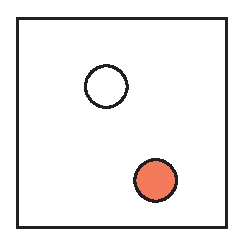
\includegraphics[width=1.5in]{images/samplefigure}
%%   \caption{Sample illustration.}
%% \end{figure}

\section{Methods}

In games, grass is usually simulated by rendering billboards. The billboards are then animated by transforming the top vertices to have wind-like movement. While this is a very simple approach that works well in games since processing and graphics power is needed elsewhere, it does not yield stunning visuals. This paper focuses on a different approach, where each grass blade has full geometry and can be completely animated. It puts high value on putting the workload on the GPU instead of the CPU by mainly making use of the geometry shader.

\subsection{Generating grass grid}
The grass grid is generated by laying down root points as can be seen in Figure {?}. First, a grid of patches is created and each patch generates its own root points. Using a density map {Figure ?} that is equal the size of the terrain height map, local density spots can be adjusted. All root points are pushed into a single vertex buffer object and can be, in theory, rendered with a single draw call. However, the patches are used to achieve several things:

\begin{description}
  \item[Culling] \hfill \\
  A single patch can be visualized by a bounding box, which can then be easily checked against the view frusrum to cull patches outside of it. It is important to take the grass animation into account when creating the bounding box - otherwise grass could be culled when moving into the frustum.
  \item[Level of detail] \hfill \\
  The distance from the camera to the mid point of a patch can be calculated and used to set the level of detail. This saves a few instructions as level of detail does not have to be calculated within the geometry shader, thus making it possible to use geometry shaders that are pre-compiled with a static vertex count, which will improve performance.
  \item[Further individualization] \hfill \\
	It's possible to pass options into the shaders for rendering a patch, which can be used for wind animation, grass height or any other property of the grass.
\end{description}

\subsection{Terrain}
The terrain is generated out of a height map, which was generated by Perlin Noise. We can map the grass root position to our terrain grid to find the matching Y position. It is important to take the density of the grass into account when calculating lighting of the terrain. Using the density map, we can darken areas where grass is very dense - easily simulating ambient occlusion.

[INSERT picture of terrain with grass on it]

\subsection{Generating the blade}
The geometry shader needs to be able to generate grass blades with a different level of detail. Instead of writing separate geometry shaders, we decided to write one geometry shader that prodecurally generates the blade. When generating the blade, we want to concentrate the vertices on the top half of the blade to have a smooth animation later on. It is also needed to calculate the UV-coordinate, normals and rotation, as well as vertex displacement for wind later on.

A visual representation of the algorithm can be seen in Figure {?}

\subsection{Pipeline}
To summarize, this is a list of important components in our project and their respective job.
\begin{description}
  \item[CPU] \hfill \\
  The CPU will generate the root points out of the density map and create a single vertex buffer, that contains all roots. It will also slice the full grass grid into smaller patches, which can be controlled through constant buffers on the GPU.
  
  Since we also have static terrain, the root points will already contain the correct displaced Y position.
  \item[Vertex shader] \hfill \\
  The vertex shader is, in essence, a pass-through shader.
  \item[Geometry shader] \hfill \\
  All the hard work is done in the geometry shader. Since the geometry shader gets a single point as an input, it's job is to create a grass blade with a specified number of vertices. The geometry shader will also take care of calculating normals, level of detail, and animation.
  \item[Pixel shader] \hfill \\
  To calculate the color, we use the basic Phong BDRF, combined with a texture and a randomized tint.
\end{description}

\subsection{Flickering}
A very prevalent problem while implementing this approach was flickering. Due to the high amount of very thin grass blades, blades were fighting for pixels and a lot of aliasing and flickering could be seen. In order to minimize this effect, several techniques were used:

Explain: Width and height influence, density changes, downsampling.

\section{Randomization}

The scene looks very artificial if the grass is laid out with exact distances, when each grass blade has the same tint, height or width. However, it is fairly difficult to generate random numbers on the GPU, which is why we have to use certain tricks to have fairly random grass properties. When laying out the root points, we can generate random positions using the CPU.

Since these root points are given to the geometry shader, and we kow that these positions are random, we can generate a random number between -1 and 1 using the following equation.

\begin{equation}
r = sin(\frac{\pi}2 * frac(root.x) + \frac{\pi}2 * frac(root.z))
\end{equation}

[INSERT non-randomized and randomized picture]

Using this randomized value, several grass properties can be influenced. Some of those are: width, height, color tint, rotation, wind.

\section{Animation}
Explain: Basic sine animation, Wind, Oscillation, Wind field
For animating the grass blades, a simulation of wind is used to achieve a realistic look. In order to maximize the interactivity, the user should be able to influence wind speed and direction. 

In general, the wind simulation consists of two components:

\begin{description}
  \item[Vertex displacement] \hfill \\
  This components takes care of simulation the effect of wind hitting a single blade, which displaces the mesh.
  \item[Wind field simulation] \hfill \\
  To simulate the effect of wind over a field of grass, a 2D wind field is used.
\end{description}

\subsection{Vertex displacement}


\subsection{Wind field simulation}

\section{Wheat differences}
Explain: Flat plane does not work very well.

\section{Benchmarks}
We kept randomized values to a minimum to avoid variations in the scene and to have a baseline. All tests were mainly done on the following two systems.

\begin{flushleft}
\begin{description}
  \item[System 1 (Desktop)] \hfill \\
  CPU: Intel Xeon E5-1230v3 \linebreak
  RAM: 16GB DDR3-1333 \linebreak
  GPU: nVidia GeForce GTX 780
  \item[System 2 (Notebook)] \hfill \\
  CPU: Intel Core I7-4980HQ \linebreak
  RAM: 16GB DDR3-1333 \linebreak
  GPU: Intel Iris Pro
\end{description}
\end{flushleft}

Content: Show base FPS without performance improvements, then show level of detail, culling and so on.

\section{Shortcomings and improvements}

As shown in the section "Benchmarks", this approach does not need high-end processing power as of todays standards. Using 1 million grass blades, the implementation can be run on integrated graphics cards on Notebooks with 60 FPS.

The main visual problem is flickering. Using native resolution of displays and no anti-aliasing, the thin blades cause a lot of flickering in the distance - even when using the tricks described in the paper to minimize it. However, when rendered on a high PPI screen or by using techniques like Downsampling[?], flickering vanishes very fast.

\bibliographystyle{acmsiggraph}
\bibliography{template}
\end{document}
